%!TEX root = ../MasterThesis.tex

\section{Overview}
\label{sec:system_overview}

Based on the explanations in Section~\ref{cha:context_analysis}, and especially the scope definition for this Master thesis in Section~\ref{sec:scope_thesis}, the system for investigating E-commerce fraud incidents have to answer the central question:\@

\begin{quotation}
    \textit{Is this really a fraudulent E-commerce transaction?}
\end{quotation}

The main stakeholders, that need to be involved in the investigation process are:\@

\begin{itemize}
    \item the online merchants
    \item the \gls{PSP}
    \item the issuer
\end{itemize}

Ideally they would make part of their internal information available for external partners to access and query for, so that the party, who has to authorize or validate the credit card payment can analyse all available information, as depicted in the Figure~\ref{fig:images_system_overview}.

\begin{figure}[H]
	\centering
		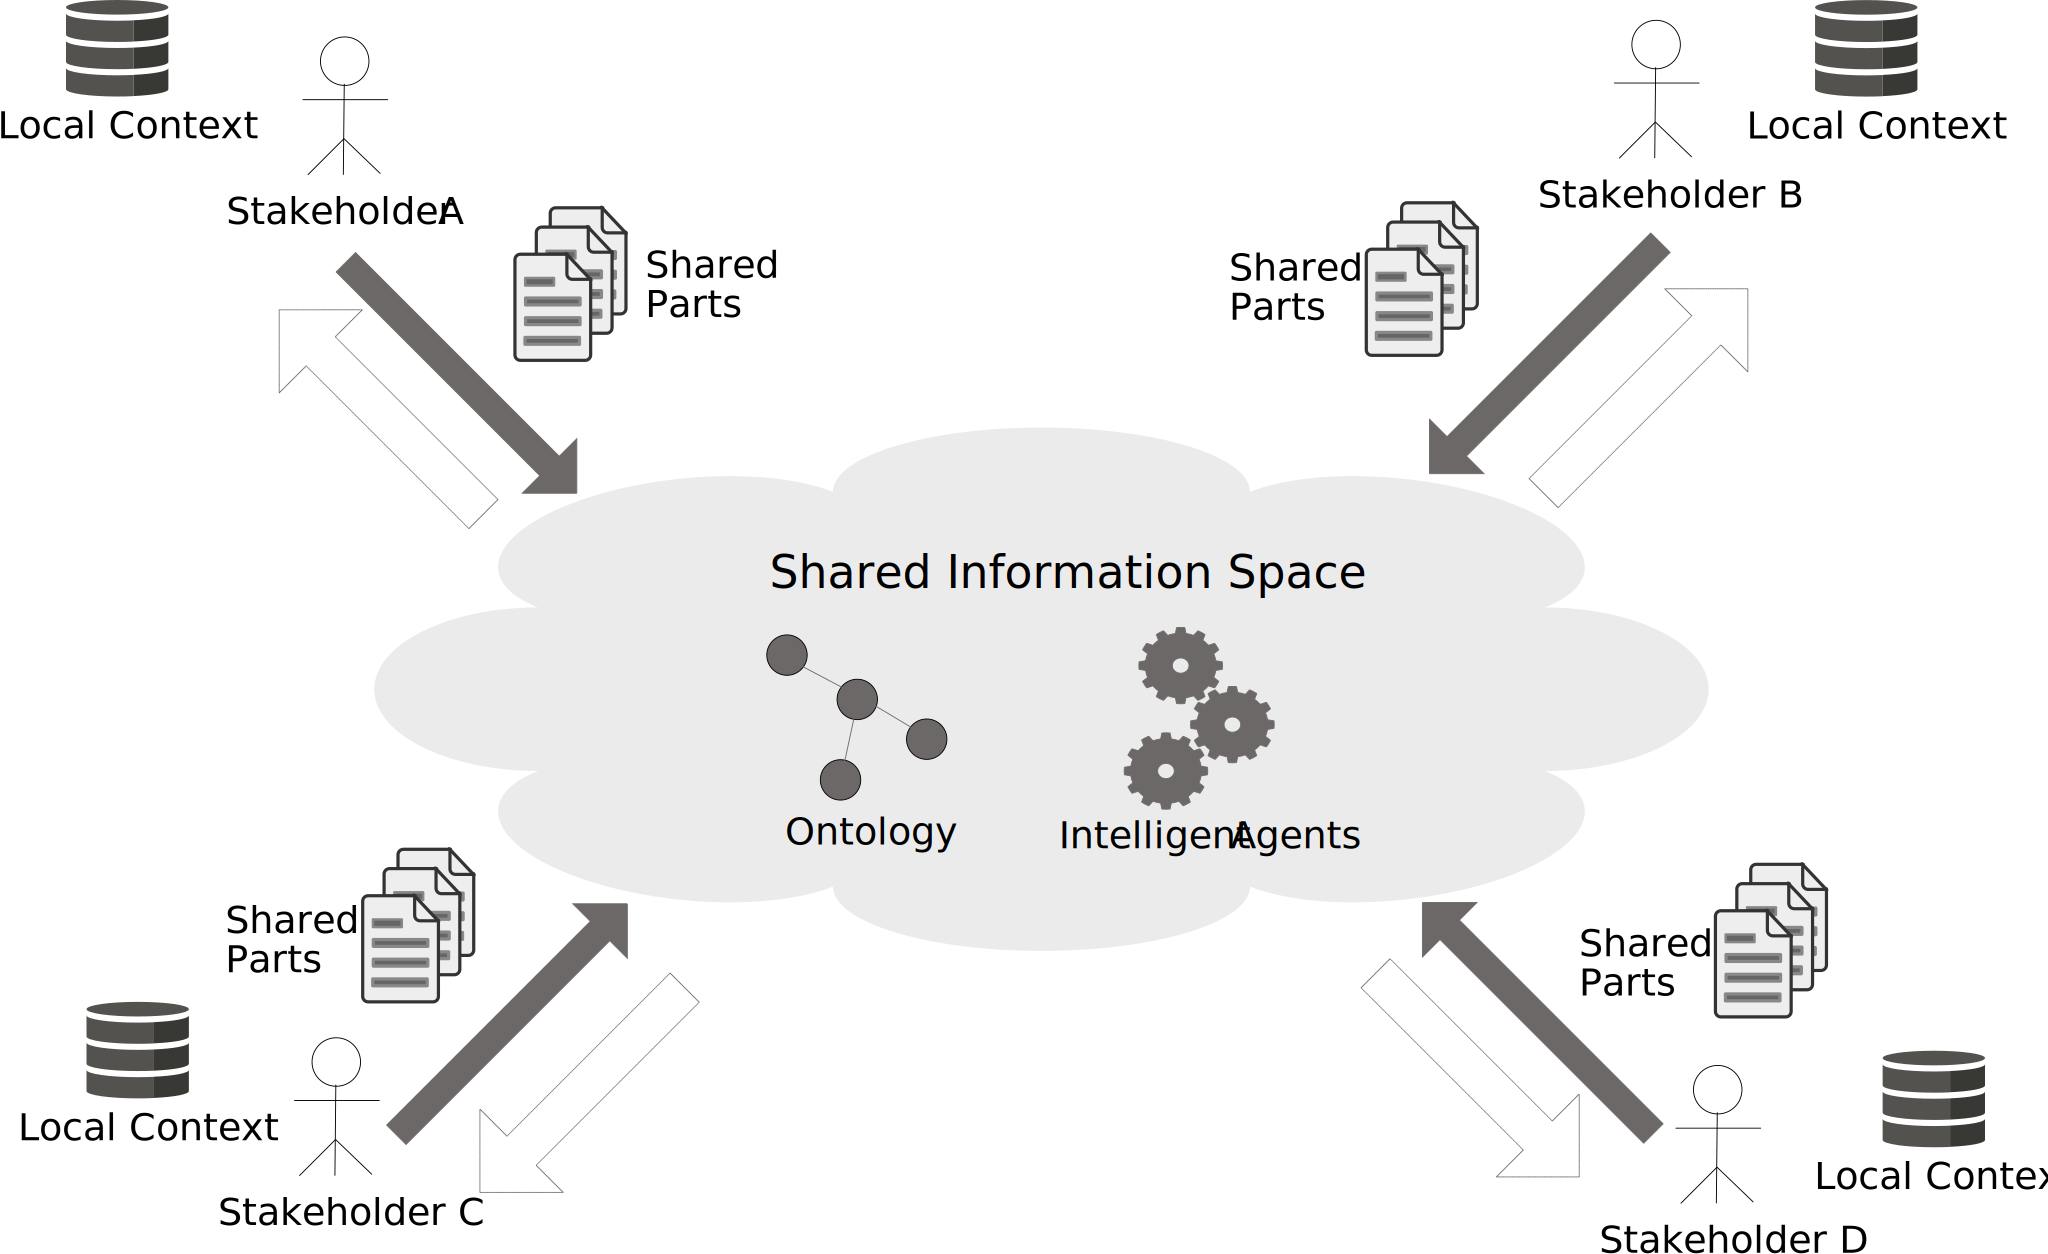
\includegraphics[width=0.8\columnwidth]{images/system_overview.pdf}
	\caption{System Overview}
\label{fig:images_system_overview}
\end{figure}

\ldots


\begin{figure}[H]
	\centering
		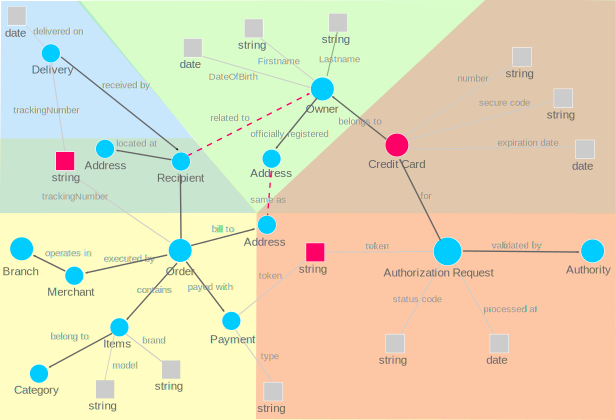
\includegraphics[width=0.8\columnwidth]{images/ontology_scenario_1.pdf}
	\caption{Data Model}
\label{fig:images_data_model}
\end{figure}


% section system_overview (end)
